% Chapter Template

\chapter{Secure Compartmentalisation} % Main chapter title

\label{Chapter 6} % Change X to a consecutive number; for referencing this chapter elsewhere, use \ref{ChapterX}

This chapter goes over the frame work for how secure compartments will be implemented in the MEGA65. It will then discuss the problems encountered during the implementation of the secure compartments. Finally this chapter will talk about the possible issues with the secure compartments.

%----------------------------------------------------------------------------------------
%	SECTION 1
%----------------------------------------------------------------------------------------

\section{Theorised Operation}

\label{Ch6 Sec1}

Thanks to the work of Tim Kirby, a frame work was provided for the operation of the secure compartments of the phone, as seen in figure \ref{fig:timkirby}. From this diagram, the finite state machine seen in figure \ref{fig:securecompartmentsfsm} was created and the state transition actions were noted. As seen in both figures \ref{fig:timkirby} and \ref{fig:securecompartmentsfsm}, initially the user begins in the insecure user mode. This user mode is then halted via a hypervisor trap that causes the io registers and the RAM and ROM of the phone to be saved to the SD card. The non-transfer section of RAM and all of ROM are then erased. From one of the save-state slots on the SD card, the desired secure service is then loaded into ROM. As soon as this is finished matrix mode is triggered, the hypervisor is left and the CPU is halted. Matrix mode causes all external input into the phone, apart from the keyboard, to be cut off. At this point the user is able to inspect ROM and the transfer area of RAM. If the user is satisfied, by typing "ACCEPT" the secure service is then allowed to execute with the data provided in the transfer area of RAM. If the user is dissatisfied, by typing "REJECT" the secure service is erased from ROM, matrix mode is then left, the hypervisor is retriggered and the CPU is resumed. The hypervisor then uses the save-state created immediately prior to entering matrix mode to restore the io registers and load all the data that was saved back into RAM and ROM. If the secure container was accepted, any additional trap to the hypervisor will be seen as an exit request from the secure container. During an exit request, the user will once again be prompted to inspect the transfer area of RAM and then accept or reject the escaping of the of that data from the secure container. If satisfied, by typing "ACCEPT" the non-transfer section if RAM and all of ROM are once again erased. Then, identically to the user rejecting entry into the secure container, matrix mode is left, the hypervisor is retriggered and the CPU is resumed. The hypervisor then loads the save-state created immediately prior to entering matrix mode from the SD card, which is used to restore the io registers and reload data back into non-transfer RAM and ROM. If the user is dissatisfied with data escaping the secure container, by typing "REJECT" all of RAM and all of ROM are erased before the matrix mode exit. Then the save-state is loaded identically to the accepted exit case by the hypervisor and the resumed CPU. Finally, an exit status flag is raised depending on how the secure service transaction went.

\begin{figure}
  \centering
  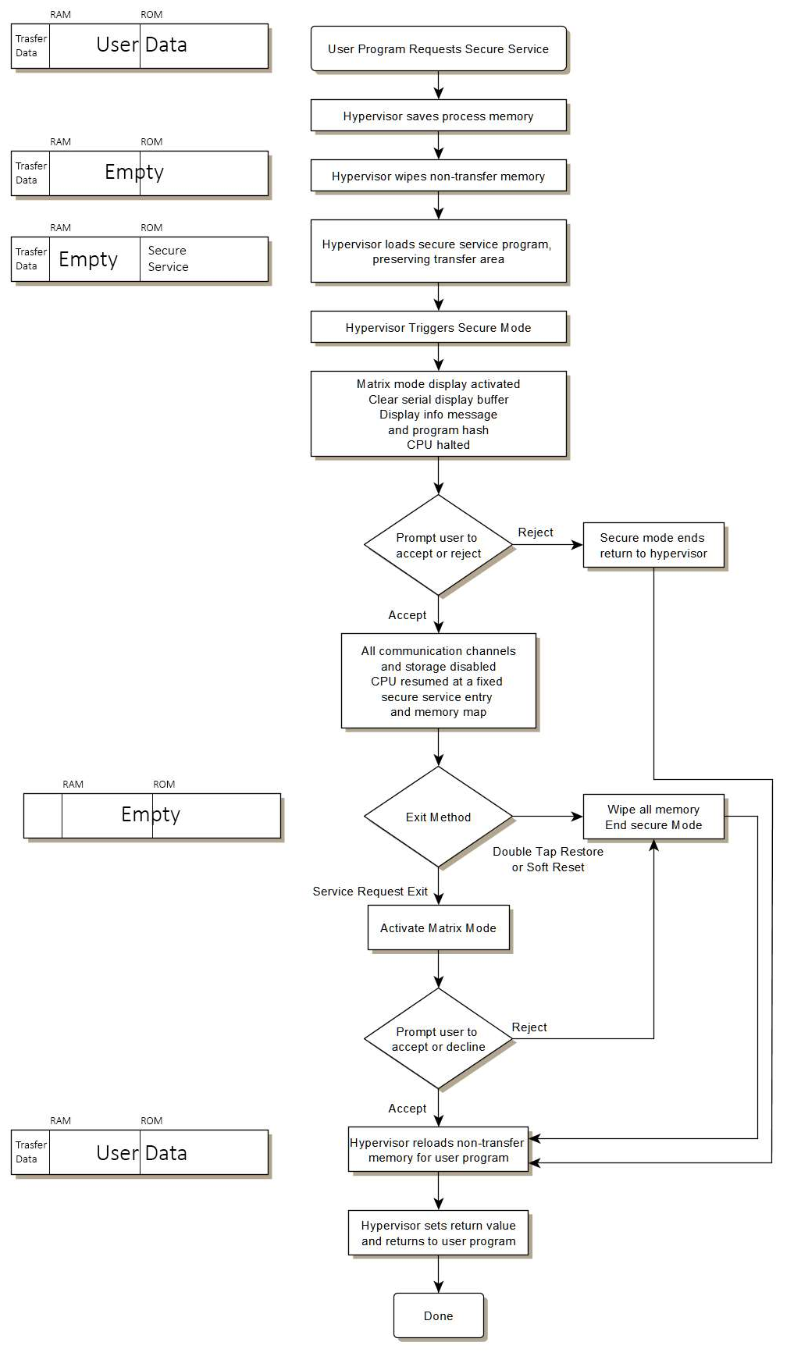
\includegraphics[width=\linewidth]{timkirby}
  \caption{The secure compartment frame work provided by Tim Kirby's thesis "Design and Development of a Secure Compartmentalised 8-bit Architecture".}
  \label{fig:timkirby}
\end{figure}

\begin{figure}
  \centering
  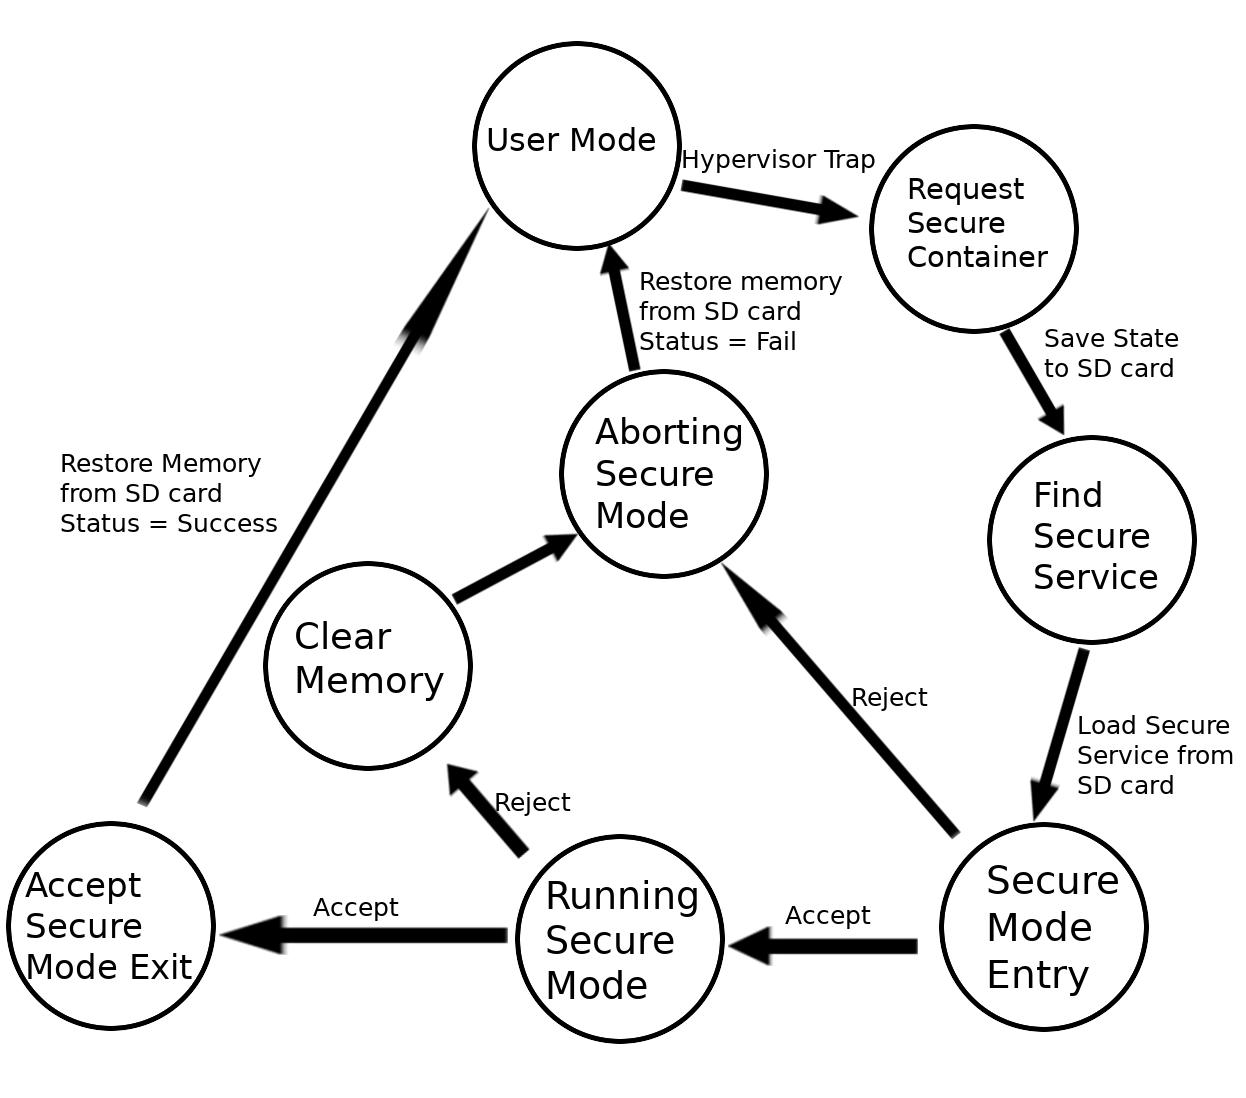
\includegraphics[width=\linewidth]{securecompartmentfsm}
  \caption{}
  \label{fig:securecompartmentsfsm}
\end{figure}

%----------------------------------------------------------------------------------------
%	SECTION 2
%----------------------------------------------------------------------------------------

\section{Initial Issues}

\label{Ch6 Sec2}

As the secure compartments were entirely separate from the matrix mode corrections and during the time a major update for another section of the phone was finished, a new branch of the project was created. Switching to this new branch resulted in overhead issues that needed to be solved in order for the project to proceed further.

%-----------------------------------
%	SUBSECTION 1
%-----------------------------------
\subsection{Repairing the Branch}

\label{Ch6 Sec2 Sub1}

As a new section of the project was being worked on the by other developers in isolation from the changes I had made, many of the fixes I had implemented had to be redone.\\
The timing fixes done to possibly correct the matrix mode issue were all removed, including the generation of the timing reports, these were reimplemented. The implementation was identical to that described in section \ref{Ch5 Sec1 Sub2} of chapter \ref{Chapter 5}.\\
All of the letterboxing changes were lost, so, as seen in section \ref{Ch5 Sec2} of chapter \ref{Chapter 5}, the erasing of the second character set was done one gains and the letterbox signal was one again used to limit the output of matrix mode.\\
The revolving line issue due to discrepancies in line length returned as was fixed as described in section \ref{Ch5 Sec3 Sub1} of chapter \ref{Chapter 5}.\\

In addition to the minor issues, matrix mode was not behaving as intended again. When attempting to enter or exit matrix mode with the tab + C= key combination, the key combination would be read and re-read rapidly and continuously. This made entering and exiting matrix mode unreliable as it was up to luck whether the key combination was scanned an odd or even amount of times to determine if the state was toggled. Tracing the matrix mode hypervisor trap from the CPU to the io mapper shows, as seen in figure \ref{fig:mmlatch}, there are latching and unlatching conditions for the matrix mode hypervisor trap. When monitoring the ascii\_key\_valid and ef\_latch signals via oscilloscope, the cause of the issue was clear. The ascii\_key\_valid signal was not a latching signal, and thus, it would only be high for a single clock cycle. As seen in the logic in figure \ref{fig:mmlatch}, this would cause the latch signal to pulse similarly, allowing the matrix mode hyper trap to be triggered every second clock cycle. A quick solution to this issue, as seen in figure \ref{fig:traptimeout} was written by Dr. Gardner-Stephen in the form of a timeout clock that blocks repeated instances of tab + C= from triggering the matrix mode hypervisor trap.

\begin{figure}
  \centering
  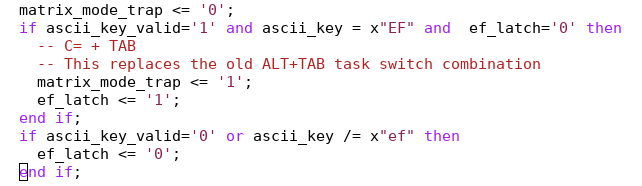
\includegraphics[width=\linewidth]{mmlatch}
  \caption{The matrix mode hypervisor trap latch.}
  \label{fig:mmlatch}
\end{figure}

\begin{figure}
  \centering
  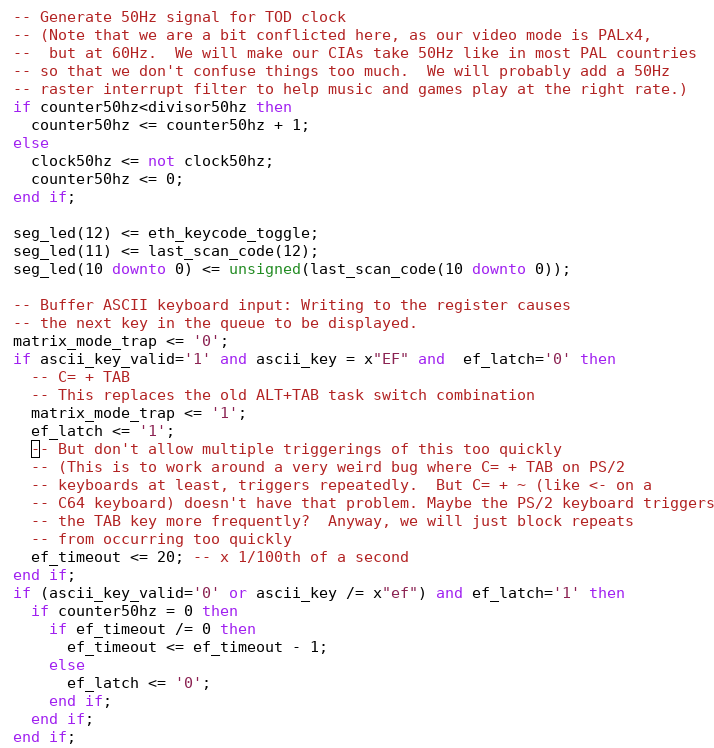
\includegraphics[width=\linewidth]{traptimeout}
  \caption{The matrix mode hypervisor trap latch with the new timeout period to prevent constant triggering.}
  \label{fig:traptimeout}
\end{figure}

%-----------------------------------
%	SUBSECTION 2
%-----------------------------------
\subsection{SD Card Restoration}

\label{Ch6 Sec2 Sub2}

One of the already implemented functions on the phone was the freeze function, this allowed the user to save state to a "Slot" located on the SD card. This freeze function would be the basis for the saving to and loading from the SD card when entering and exiting secure mode. The functionality for the standard capacity SD cards (SDSC) was entirely as expected, it was only the high capacity SD cards (SDHC) that were causing issues. When attempting to write to an SDHC card with the existing code, no visible errors occurred. It was only when attempting to read from this card that an issue occurred. When attempting to read after the first time the SD card would read no data, each read required a reset of the SD card between them in order for correct functionality. The extreme capacity SD card (SDXC) was not supported by the current hardware and indeed, was not recognised as an SD card at all when reading and writing was attempted. At the suggestion of Dr. Garner-Stephen, the issue with the SDHC cards was examined from the finite state machine located in the sdcard.vhdl file. As seen in figure \ref{fig:sdcardread} when reading or writing, the SD card is selected by making the cs\_bo bit low, and when it is not doing either of them, it is deselected by making cs\_bo high. Comparing this to the reset process seen in figures \ref{fig:resetsdcard}, \ref{fig:startsdcard} and \ref{fig:deselectsdcard}, it can be seen that there are several signals that are not being propagated when deselecting the SD card. At the suggestion of Dr. Gardner-Stephen, the simple solution of not deselecting the SD card was used. This solution, as seen in figure \ref{fig:sdcardfix}, does not provide hot swapping of the SD card, but has the functionality required for the secure mode implementation.

\begin{figure}
  \centering
  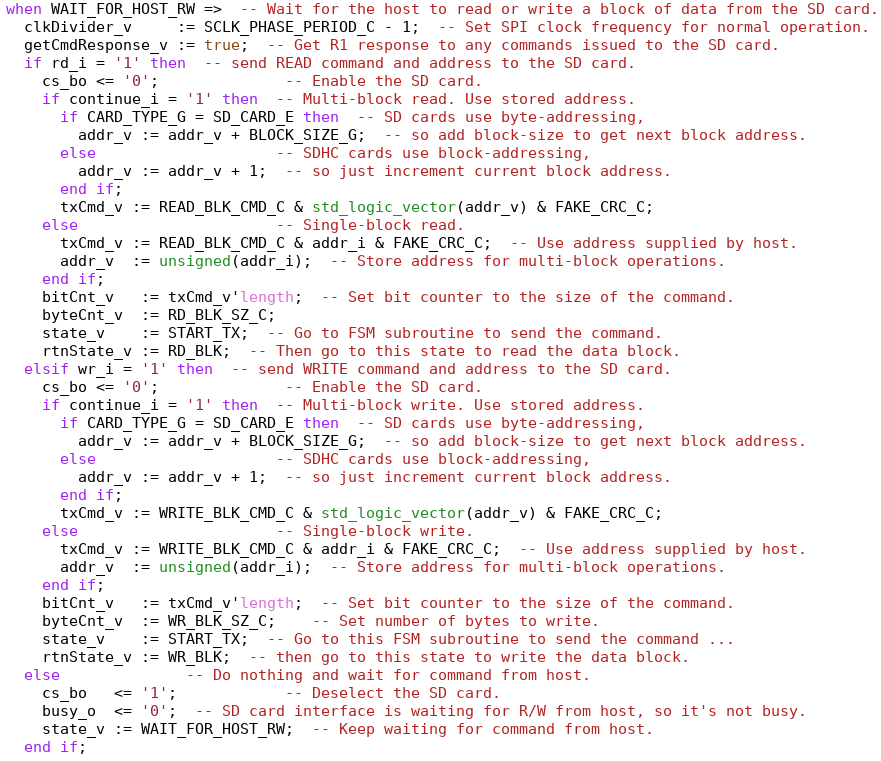
\includegraphics[width=\linewidth]{sdcardread}
  \caption{The SD card idle state code.}
  \label{fig:sdcardread}
\end{figure}

\begin{figure}
  \centering
  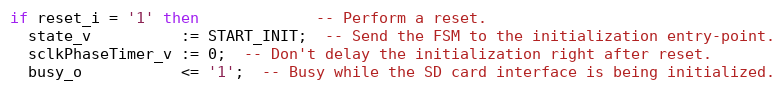
\includegraphics[width=\linewidth]{resetsdcard}
  \caption{The reset SD card code.}
  \label{fig:resetsdcard}
\end{figure}

\begin{figure}
  \centering
  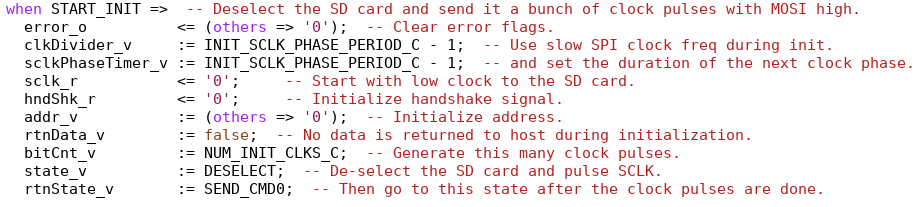
\includegraphics[width=\linewidth]{startsdcard}
  \caption{The SD card initial start up code.}
  \label{fig:startsdcard}
\end{figure}

\begin{figure}
  \centering
  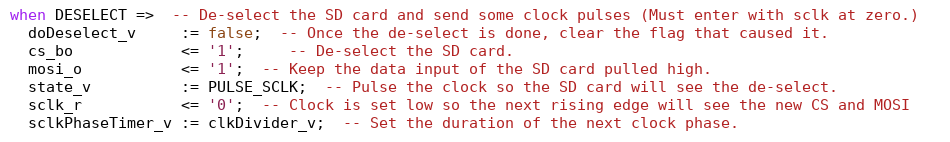
\includegraphics[width=\linewidth]{deselectsdcard}
  \caption{The deselect SD card code.}
  \label{fig:deselectsdcard}
\end{figure}

\begin{figure}
  \centering
  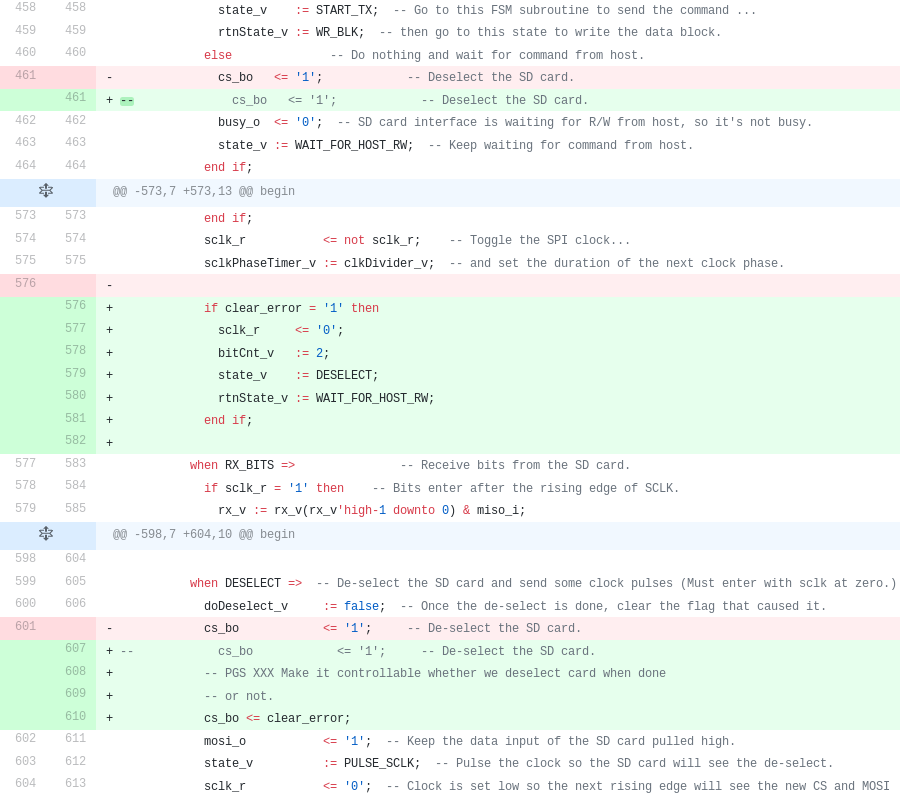
\includegraphics[width=\linewidth]{sdcardfix}
  \caption{The fixed read, write and idle code for the SD card controller.}
  \label{fig:sdcardfix}
\end{figure}

%----------------------------------------------------------------------------------------
%	SECTION 3
%----------------------------------------------------------------------------------------

\section{Secure Compartment Implementation}

\label{Ch6 Sec3}

%-----------------------------------
%	SUBSECTION 1
%-----------------------------------

\subsection{Secure Mode Trap}

\label{Ch6 Sec3 Sub1}

As discussed in section \ref{Ch6 Sec1}, in order for the user to enter secure mode a hypervisor trap needs to be sent to the CPU. All hypervisor traps work in a single standard way, a set of conditions, usually a key combination, pulls the hypervisor trap signal low. This signal is then fed out of the triggering hardware where it is combined with the the other hypervisor traps to form a singular, active low, hypervisor trap. This hypervisor trap signal, seen in figure \ref{fig:hypervisortrap}, is then sent to the CPU, where it is used to determine the type of hypervisor trap occurring. As seen in figure \ref{fig:hypertrappending}, this trap input is then used to generate an edge signal which is further used to latch the hypervisor trap pending signal. This prevents the hypervisor trap from being lost if not active for long enough. This is then used in figure \ref{fig:enterhypervisor} to cause the next instruction of the CPU to enter the hypervisor mode. When entering the hypervisor the secure mode bit is checked to see if secure mode is already active, this is used for exiting secure mode and further discussed in section \ref{Ch6 Sec3 Sub4}. As seen in figure \ref{fig:hypertraptype}, when not in secure mode, the hypervisor\_trap\_port signal is used as a pointer to set the program counter to the desired hypervisor trap location in memory. These memory locations start at \$8000 and the secure mode trap is trap 11, which starts at memory location \$8044 and can be seen in figure \ref{fig:hypertrapsoftware}. This location in memory is where the next stage of the secure mode process, as described in section \ref{Ch6 Sec3 Sub2}, will take place.

\begin{figure}
  \centering
  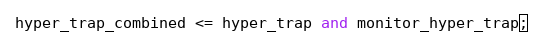
\includegraphics[width=\linewidth]{hypervisortrap}
  \caption{The combining of the keyboard hypervisor trap and the monitor hypervisor trap.}
  \label{fig:hypervisortrap}
\end{figure}

\begin{figure}
  \centering
  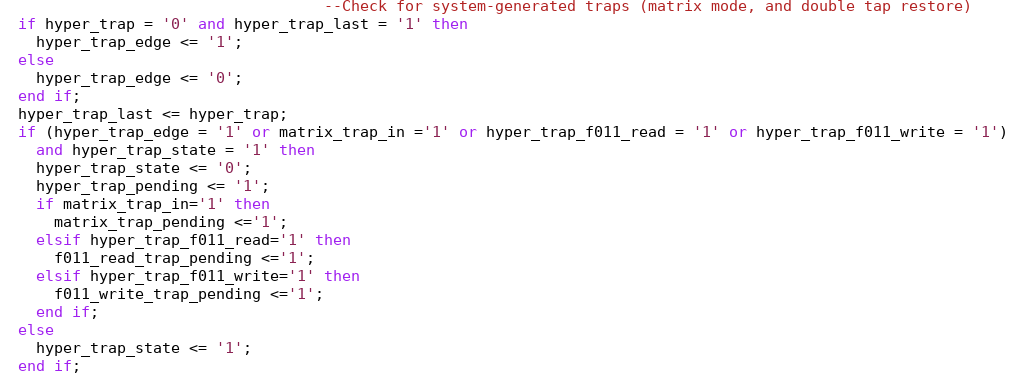
\includegraphics[width=\linewidth]{hypertrappending}
  \caption{The hypervisor trap edge generation, pending trap generation and special trap input generation.}
  \label{fig:hypertrappending}
\end{figure}

\begin{figure}
  \centering
  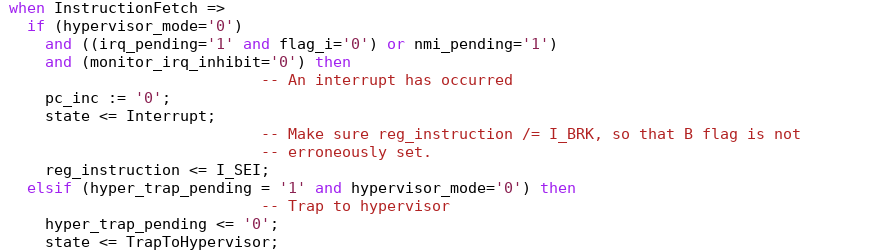
\includegraphics[width=\linewidth]{enterhypervisor}
  \caption{The use of the hyper\_trap\_pending flag to enter the hypervisor mode.}
  \label{fig:enterhypervisor}
\end{figure}

\begin{figure}
  \centering
  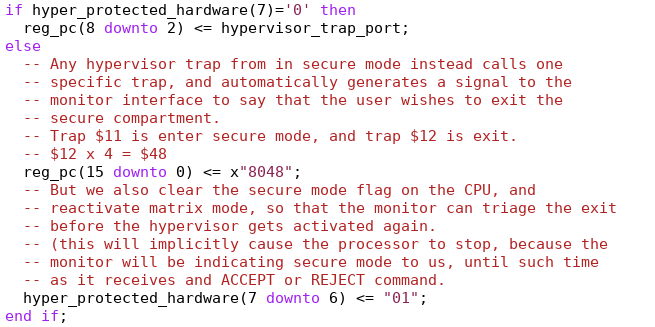
\includegraphics[width=\linewidth]{hypertraptype}
  \caption{The statement that determines the type of hypervisor trap while entering hypervisor mode.}
  \label{fig:hypertraptype}
\end{figure}

\begin{figure}
  \centering
  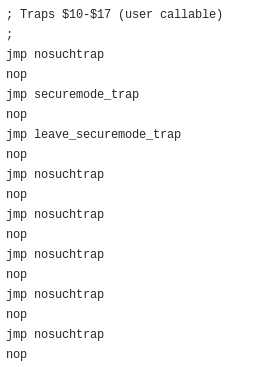
\includegraphics[width=\linewidth]{hypertrapsoftware}
  \caption{The secure mode hypervisor trap service call.}
  \label{fig:hypertrapsoftware}
\end{figure}

%-----------------------------------
%	SUBSECTION 2
%-----------------------------------

\subsection{Save and Load State}

\label{Ch6 Sec3 Sub2}

Once trapped to the hypervisor, as described in section \ref{Ch6 Sec1} and seen in figure \ref{fig:timkirby}, the io registers, RAM and ROM all need to be saved to a save state slot. Upon entering the hypervisor, as seen in figure

\begin{figure}
  \centering
  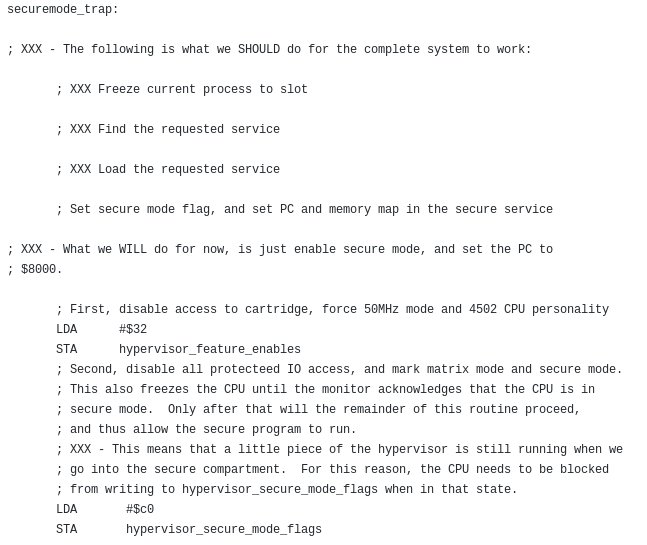
\includegraphics[width=\linewidth]{hypertrapsoftwareone}
  \caption{}
  \label{fig:hypertrapsoftwareone}
\end{figure}

\begin{figure}
  \centering
  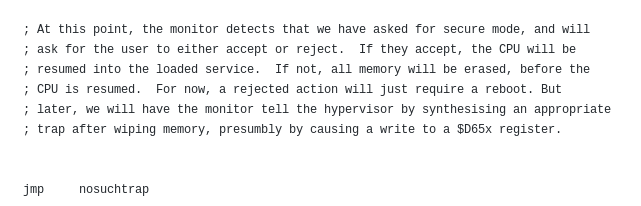
\includegraphics[width=\linewidth]{hypertrapsoftwaretwo}
  \caption{}
  \label{fig:hypertrapsoftwaretwo}
\end{figure}

%-----------------------------------
%	SUBSECTION 3
%-----------------------------------

\subsection{Secure Mode Entry}

\label{Ch6 Sec3 Sub3}

With the io registers, RAM and ROM all saved and the secure service loaded into RAM and ROM while preserving the transfer area, entry into secure mode can begin. This starts with the hypervisor toggling the secure mode and matrix mode bits of the protected hardware flags. As soon as there is a mismatch between the monitor secure mode flag and the CPU secure mode flag, as seen in figure \ref{fig:cpuhalt} the CPU is halted. This allows the secure mode signal to propagate out of the CPU to the monitor.\\

The monitor, as opposed to the Intel Management Engine (IME) service CPU, is a servant CPU. The key difference between the two being that where the IME is able to autonomously perform commands, whereas the monitor CPU requires the user to issue commands. The monitor CPU was introduced due to hardware limitations of the FPGA. Previously the monitor was entirely hardware with no CPU at all, this took up lots of space on the FPGA and would prevent the rest of the phone from being able to fit. By converting the monitor into a servant CPU the large amount of specialised hardware was able to be condensed into a multipurpose unit.\\

As seen in figure \ref{fig:monitorprotectedhardware}, when the secure mode flag reaches the monitor CPU, it is eventually scanned and used to branch and enter the secure mode routine. In this routine, as seen in figure \ref{fig:maybeentersecuremode}, currently only the local secure mode variable is set high and the routine returns to figure \ref{fig:monitorprotectedhardware}. In the future iterations, an indicator as to how much memory the transfer area occupies will need to be implemented.\\

In parallel to the monitor functions, the protected hardware signal is fed into the matrix mode compositor. This displays the secure mode screen entirely independently from the secure mode verification and locks down the inputs and outputs from the MEGA65. Once the monitor CPU verification has completed, as seen in figure \ref{fig:monitoracceptreject} the user is required to enter "ACCEPT" or "REJECT" to approve or disapprove entry into the secure container. In the "ACCEPT" case, this will parse the local secure mode variable out and to the CPU. In the "REJECT" case, the io registers, RAM and ROM are be restored from the save state created in section \ref{Ch6 Sec3 Sub3} and then the local variable for secure mode will be parsed to the CPU. The "ACCEPT" case can be seen in figure \ref{fig:monitoraccept} and the "REJECT" case can be seen in figure \ref{fig:monitorreject}.\\

While the "ACCEPT" case has been fully implemented, the "REJECT" case has not been implemented at all. Figure \ref{fig:monitorreject} shows that in the "REJECT" case, all that is occuring is the memory is being erased. Once the memory has been erased, the "REJECT" case continues on into the "ACCEPT" case where the local secure mode value is sent to the CPU, entering secure mode anyway. This is not how the check should function. In the future this reject command should be dependant on the state of the local secure mode bit. If this bit is high, hence we are attemping to enter secure mode, then memory should not be erased. The "REJECT" case should instead retrigger the hypervisor and bypass the exit secure mode confimration, causing the hypervisor to reload the save state created in section \ref{Ch6 Sec3 Sub2} once the CPU is resumed.\\

Once the input has been read and either the "ACCEPT" case or the "REJECT" case has been recognised and acted upon, the monitor will then leave the matrix mode screen, as seen in figure \ref{fig:monitoraccept}. In addition to leaving the matrix mode screen, the CPU is unhalted, this allows the secure service or loaded save state to function.

\begin{figure}
  \centering
  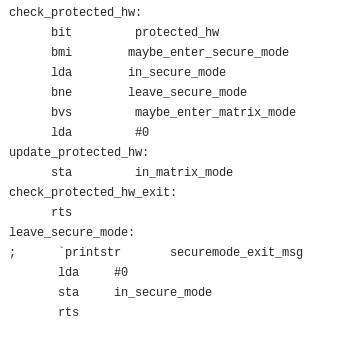
\includegraphics[width=\linewidth]{monitorprotectedhardware}
  \caption{The routine that checks the protected hardware to determine if the phone should be in secure mode}
  \label{fig:monitorprotectedhardware}
\end{figure}

\begin{figure}
  \centering
  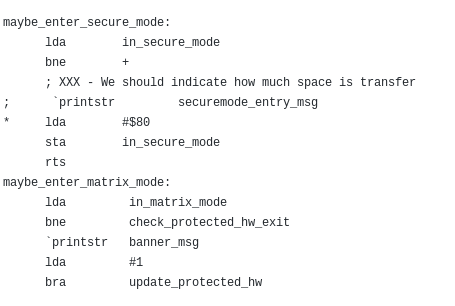
\includegraphics[width=\linewidth]{maybeentersecuremode}
  \caption{The routine that sets the secure mode flag to non-zero value.}
  \label{fig:maybeentersecuremode}
\end{figure}

\begin{figure}
  \centering
  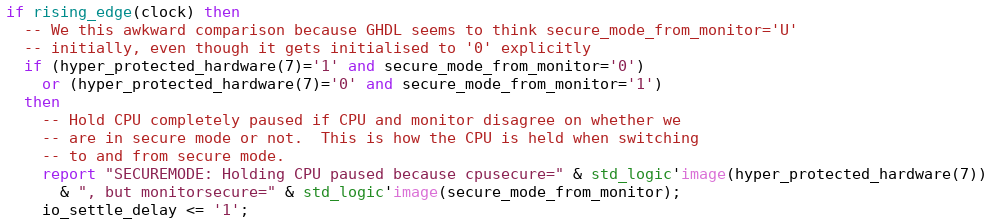
\includegraphics[width=\linewidth]{cpuhalt}
  \caption{The CPU halting code that halts when the CPU and monitor disagree on if the phone is in secure mode.}
  \label{fig:cpuhalt}
\end{figure}

\begin{figure}
  \centering
  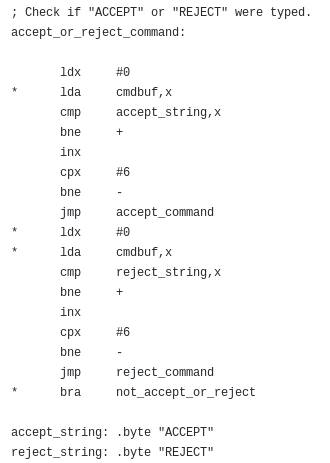
\includegraphics[width=\linewidth]{monitoracceptreject}
  \caption{The monitor CPU code that compares the input string against a string containing "ACCEPT" and one containing "REJECT".}
  \label{fig:monitoracceptreject}
\end{figure}

\begin{figure}
  \centering
  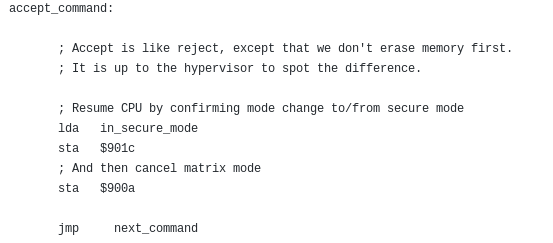
\includegraphics[width=\linewidth]{monitoraccept}
  \caption{The monitor CPU "ACCEPT" case.}
  \label{fig:monitoraccept}
\end{figure}

\begin{figure}
  \centering
  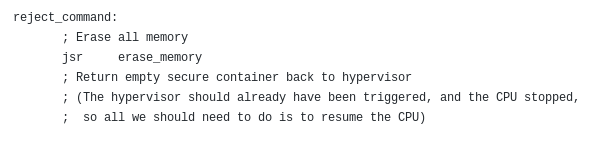
\includegraphics[width=\linewidth]{monitorreject}
  \caption{The monitor CPU "REJECT" case.}
  \label{fig:monitorreject}
\end{figure}

%-----------------------------------
%	SUBSECTION 4
%-----------------------------------

\subsection{Secure Mode Exit}

\label{Ch6 Sec3 Sub4}

While in secure mode, any hypervisor trap will be seen as a request for exit from secure mode. This, as seen in figure \ref{fig:securemodeexit}, overwrites the hypervisor trap determination seen in figure \ref{fig:enterhypervisor} with the exact location of the exit secure mode trap and sets the matrix mode flag high and secure mode flag low. Once again the CPU is halted due to the mismatch seen in figure \ref{fig:cpuhalt} between the monitor secure mode state and the CPU secure mode state.\\

The code seen in figure \ref{fig:monitorprotectedhardware} is once again run, but this time branches to figure \ref{fig:monitorleavesecuremode}. As in section \ref{Ch6 Sec3 Sub3}, while the monitor CPU is performing the verification check, the matrix mode compositor is displaying the secure mode exit screen and prompting the user to enter "ACCEPT" or "REJECT". As seen in figures \ref{fig:monitoracceptreject} and \ref{fig:monitoraccept}, in the "ACCEPT" case the CPU is allowed to run by setting the monitor secure mode state to be identical to the CPU. In the "REJECT" case, demonstraited by figure \ref{fig:monitorreject},  all the top megabyte of address space is erased and io address registers are also erased.\\

The "REJECT" case, as seen in figure \ref{fig:monitorerase}, has not entirely been implemented. Currently, the "REJECT" case is not dependant on the secure mode bit, causing it to call the erase memory function on entry or exit. In the future it needs to overwrite the transfer area RAM only when the local secure mode bit is low, hence it is leaving secure mode. Once all the erasing has been done, the "REJECT" case can continue, as implemented, into the "ACCEPT" case.\\

Like the "REJECT" case, the "ACCEPT" case needs to be fully implemented. Currently, accepting a leave request from secure mode allows all memory to escape the secure container. In future development, the io registers, ROM and non-transfer area RAM need to be erased. This, when componded with the "REJECT" case would erase all memory when rejecting exit from a secure container, but would only erase non-transfer area memory when accepting exit from a secure container. This "ACCEPT" case would also require some modification in it's current state to function differently when entering and exiting secure mode. As when entering secure mode, memory does not need to be erased. 

\begin{figure}
  \centering
  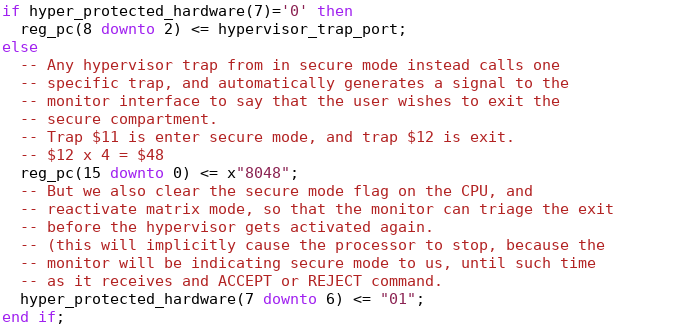
\includegraphics[width=\linewidth]{securemodeexit}
  \caption{The CPU hypervisor trap determination code.}
  \label{fig:securemodeexit}
\end{figure}

\begin{figure}
  \centering
  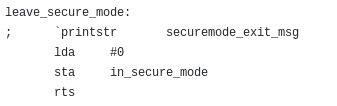
\includegraphics[width=\linewidth]{monitorleavesecuremode}
  \caption{The monitor CPU leave secure mode routine.}
  \label{fig:monitorleavesecuremode}
\end{figure}

\begin{figure}
  \centering
  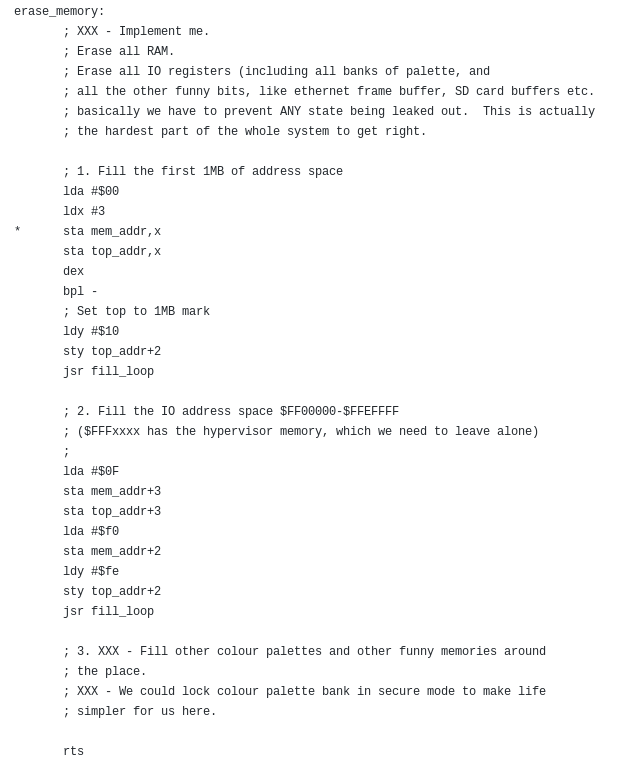
\includegraphics[width=\linewidth]{monitorerase}
  \caption{The monitor CPU erase routine.}
  \label{fig:monitorerase}
\end{figure}

%-----------------------------------
%	SUBSECTION 5
%-----------------------------------

\subsection{Restore User Mode}

\label{Ch6 Sec3 Sub5}

Once either "ACCEPT" or "REJECT" has occured and the CPU is running again, the hypervisor will then 


%% Put this in section 2

%\subsection{Secure Compartment Issue}

%\label{Ch6 Sec1 Sub1}

%During the development of the secure compartments, an issue with the design was made apparent. As explained in the previous section, when entering or exiting secure mode the hypervisor is in complete control of the phone's operation. This poses a problem if it were to experiance any subversion. Between the loading of the secure service and the entering of secure mode and halting of the CPU, there is opportunity for the 
